%%%
 % File: \activity_ratio_tikz.tex
 % Created Date: Friday, February 16th 2024
 % Author: Zihan
 % -----
 % Last Modified: Friday, 16th February 2024 11:31:29 am
 % Modified By: the developer formerly known as Zihan at <wzh4464@gmail.com>
 % -----
 % HISTORY:
 % Date      		By   	Comments
 % ----------		------	---------------------------------------------------------
%%%

\documentclass[tikz,border=10pt]{standalone}
\usepackage{tikz}
\usetikzlibrary{decorations.pathreplacing} % 加载装饰库

\begin{document}
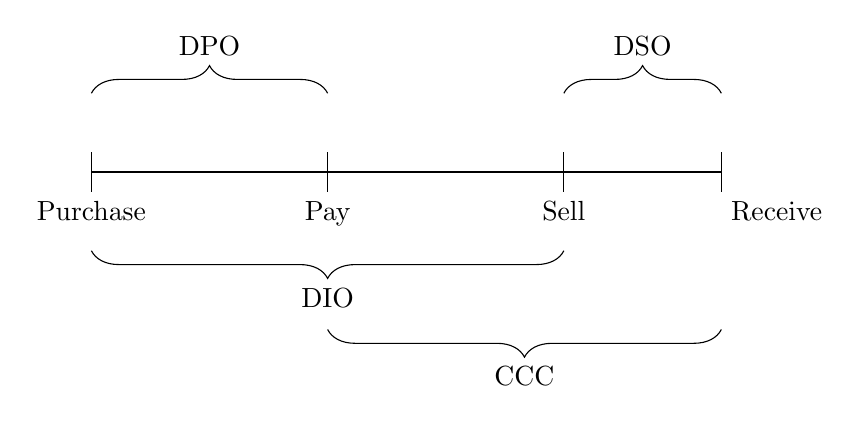
\begin{tikzpicture}

% Define the coordinates of the timeline
\coordinate (start) at (2,0);
\coordinate (end) at (10,0);

% Draw the horizontal line
\draw (start) -- (end);

% Draw the vertical lines for DIO, DSO, and DPO
\draw (2,0.25) -- (2,-0.25) node[below] {Purchase};
\draw (5,0.25) -- (5,-0.25) node[below] {Pay};
\draw (8,0.25) -- (8,-0.25) node[below] {Sell};
\draw (10,0.25) -- (10,-0.25) node[below right] {Receive};

% Draw the brackets for DPO and CCC
\draw [decorate,decoration={brace,amplitude=10pt,mirror}] (5,1) -- (2,1) 
node [black,midway,above=10pt] {DPO};
\draw [decorate,decoration={brace,amplitude=10pt}] (10,-2) -- (5,-2) 
node [black,midway,below=10pt] {CCC};
\draw [decorate,decoration={brace,amplitude=10pt}] (8,1) -- (10,1)
node [black,midway,above=10pt] {DSO};
\draw [decorate,decoration={brace,amplitude=10pt,mirror}] (2,-1) -- (8,-1)
node [black,midway,below=10pt] {DIO};

\end{tikzpicture}
\end{document}
